\documentclass{standalone}
\usepackage{tikz}
\usetikzlibrary{patterns, positioning}

\begin{document}
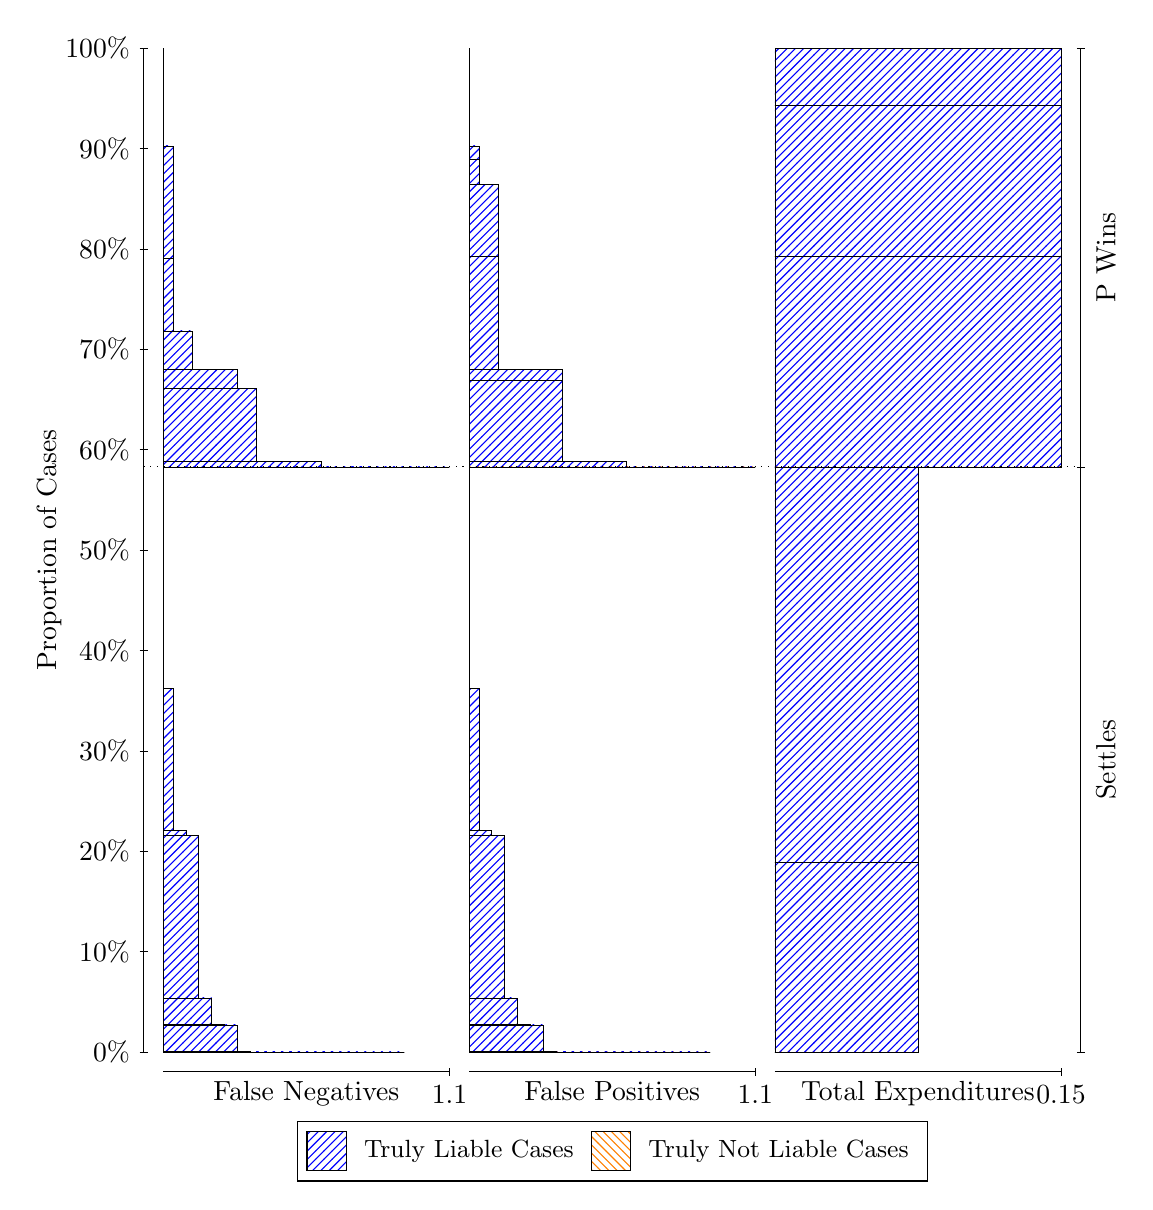
\begin{tikzpicture}
\draw[black, very thin] (1.5,1.75) -- (1.5,14.5);
\node[rotate=90, anchor=center] at (0.3, 8.125) {Proportion of Cases};
\draw[black, very thin] (1.45,1.75) -- (1.55,1.75);
\node[anchor=east] at (1.45, 1.75) {0\%};
\draw[black, very thin] (1.45,3.025) -- (1.55,3.025);
\node[anchor=east] at (1.45, 3.025) {10\%};
\draw[black, very thin] (1.45,4.3) -- (1.55,4.3);
\node[anchor=east] at (1.45, 4.3) {20\%};
\draw[black, very thin] (1.45,5.575) -- (1.55,5.575);
\node[anchor=east] at (1.45, 5.575) {30\%};
\draw[black, very thin] (1.45,6.85) -- (1.55,6.85);
\node[anchor=east] at (1.45, 6.85) {40\%};
\draw[black, very thin] (1.45,8.125) -- (1.55,8.125);
\node[anchor=east] at (1.45, 8.125) {50\%};
\draw[black, very thin] (1.45,9.4) -- (1.55,9.4);
\node[anchor=east] at (1.45, 9.4) {60\%};
\draw[black, very thin] (1.45,10.675) -- (1.55,10.675);
\node[anchor=east] at (1.45, 10.675) {70\%};
\draw[black, very thin] (1.45,11.95) -- (1.55,11.95);
\node[anchor=east] at (1.45, 11.95) {80\%};
\draw[black, very thin] (1.45,13.225) -- (1.55,13.225);
\node[anchor=east] at (1.45, 13.225) {90\%};
\draw[black, very thin] (1.45,14.5) -- (1.55,14.5);
\node[anchor=east] at (1.45, 14.5) {100\%};

\draw[black, very thin] (13.4,1.75) -- (13.4,14.5);
\draw[black, very thin] (13.35,1.75) -- (13.45,1.75);
\node[anchor=west] at (13.35, 1.75) {};
\draw[black, very thin] (13.35,9.1808) -- (13.45,9.1808);
\node[anchor=west] at (13.35, 9.1808) {};
\draw[black, very thin] (13.35,14.5) -- (13.45,14.5);
\node[anchor=west] at (13.35, 14.5) {};

\draw[black, very thin, pattern color=blue, pattern=north east lines] (1.75,1.75) rectangle (4.8118,1.75);
\draw[black, very thin, pattern color=blue, pattern=north east lines] (1.75,1.75) rectangle (4.1586,1.75);
\draw[black, very thin, pattern color=blue, pattern=north east lines] (1.75,1.75) rectangle (3.9953,1.75);
\draw[black, very thin, pattern color=blue, pattern=north east lines] (1.75,1.75) rectangle (3.5054,1.7508);
\draw[black, very thin, pattern color=blue, pattern=north east lines] (1.75,1.7508) rectangle (3.3421,1.7508);
\draw[black, very thin, pattern color=blue, pattern=north east lines] (1.75,1.7508) rectangle (3.1788,1.7513);
\draw[black, very thin, pattern color=blue, pattern=north east lines] (1.75,1.7513) rectangle (2.8522,1.7546);
\draw[black, very thin, pattern color=blue, pattern=north east lines] (1.75,1.7546) rectangle (2.689,2.0954);
\draw[black, very thin, pattern color=blue, pattern=north east lines] (1.75,2.0954) rectangle (2.5257,2.0983);
\draw[black, very thin, pattern color=blue, pattern=north east lines] (1.75,2.0983) rectangle (2.3624,2.4361);
\draw[black, very thin, pattern color=blue, pattern=north east lines] (1.75,2.4361) rectangle (2.1991,4.5019);
\draw[black, very thin, pattern color=blue, pattern=north east lines] (1.75,4.5019) rectangle (2.0358,4.5657);
\draw[black, very thin, pattern color=blue, pattern=north east lines] (1.75,4.5657) rectangle (1.8725,6.365);
\draw[black, very thin, pattern color=orange, pattern=north west lines] (1.75,6.365) rectangle (1.75,6.365);
\draw[black, very thin, pattern color=blue, pattern=north east lines] (1.75,6.365) rectangle (1.75,9.1808);
\draw[black, very thin, pattern color=blue, pattern=north east lines] (1.75,9.1808) rectangle (5.3833,9.1808);
\draw[black, very thin, pattern color=blue, pattern=north east lines] (1.75,9.1808) rectangle (4.5669,9.1819);
\draw[black, very thin, pattern color=blue, pattern=north east lines] (1.75,9.1819) rectangle (4.3219,9.1819);
\draw[black, very thin, pattern color=blue, pattern=north east lines] (1.75,9.1819) rectangle (3.7504,9.254);
\draw[black, very thin, pattern color=blue, pattern=north east lines] (1.75,9.254) rectangle (3.5054,9.2541);
\draw[black, very thin, pattern color=blue, pattern=north east lines] (1.75,9.2541) rectangle (2.9339,10.181);
\draw[black, very thin, pattern color=blue, pattern=north east lines] (1.75,10.181) rectangle (2.689,10.423);
\draw[black, very thin, pattern color=blue, pattern=north east lines] (1.75,10.423) rectangle (2.1174,10.909);
\draw[black, very thin, pattern color=blue, pattern=north east lines] (1.75,10.909) rectangle (1.8725,11.825);
\draw[black, very thin, pattern color=blue, pattern=north east lines] (1.75,11.825) rectangle (1.8725,13.258);
\draw[black, very thin, pattern color=orange, pattern=north west lines] (1.75,13.258) rectangle (1.75,13.258);
\draw[black, very thin, pattern color=blue, pattern=north east lines] (1.75,13.258) rectangle (1.75,14.5);
\draw[black, very thin, pattern color=orange, pattern=north west lines] (5.6333,1.75) rectangle (8.6951,1.75);
\draw[black, very thin, pattern color=blue, pattern=north east lines] (5.6333,1.75) rectangle (8.6951,1.75);
\draw[black, very thin, pattern color=orange, pattern=north west lines] (5.6333,1.75) rectangle (8.0419,1.75);
\draw[black, very thin, pattern color=blue, pattern=north east lines] (5.6333,1.75) rectangle (8.0419,1.75);
\draw[black, very thin, pattern color=blue, pattern=north east lines] (5.6333,1.75) rectangle (7.8787,1.75);
\draw[black, very thin, pattern color=orange, pattern=north west lines] (5.6333,1.75) rectangle (7.3888,1.75);
\draw[black, very thin, pattern color=blue, pattern=north east lines] (5.6333,1.75) rectangle (7.3888,1.7508);
\draw[black, very thin, pattern color=blue, pattern=north east lines] (5.6333,1.7508) rectangle (7.2255,1.7508);
\draw[black, very thin, pattern color=blue, pattern=north east lines] (5.6333,1.7508) rectangle (7.0622,1.7513);
\draw[black, very thin, pattern color=orange, pattern=north west lines] (5.6333,1.7513) rectangle (6.7356,1.7513);
\draw[black, very thin, pattern color=blue, pattern=north east lines] (5.6333,1.7513) rectangle (6.7356,1.7546);
\draw[black, very thin, pattern color=blue, pattern=north east lines] (5.6333,1.7546) rectangle (6.5723,2.0954);
\draw[black, very thin, pattern color=blue, pattern=north east lines] (5.6333,2.0954) rectangle (6.409,2.0983);
\draw[black, very thin, pattern color=blue, pattern=north east lines] (5.6333,2.0983) rectangle (6.2457,2.4361);
\draw[black, very thin, pattern color=orange, pattern=north west lines] (5.6333,2.4361) rectangle (6.0824,2.4361);
\draw[black, very thin, pattern color=blue, pattern=north east lines] (5.6333,2.4361) rectangle (6.0824,4.502);
\draw[black, very thin, pattern color=blue, pattern=north east lines] (5.6333,4.502) rectangle (5.9191,4.5658);
\draw[black, very thin, pattern color=blue, pattern=north east lines] (5.6333,4.5658) rectangle (5.7558,6.3651);
\draw[black, very thin, pattern color=blue, pattern=north east lines] (5.6333,6.3651) rectangle (5.6333,9.1808);
\draw[black, very thin, pattern color=orange, pattern=north west lines] (5.6333,9.1808) rectangle (9.2667,9.1808);
\draw[black, very thin, pattern color=blue, pattern=north east lines] (5.6333,9.1808) rectangle (9.2667,9.1808);
\draw[black, very thin, pattern color=orange, pattern=north west lines] (5.6333,9.1808) rectangle (8.4502,9.1808);
\draw[black, very thin, pattern color=blue, pattern=north east lines] (5.6333,9.1808) rectangle (8.4502,9.1819);
\draw[black, very thin, pattern color=orange, pattern=north west lines] (5.6333,9.1819) rectangle (7.6337,9.1819);
\draw[black, very thin, pattern color=blue, pattern=north east lines] (5.6333,9.1819) rectangle (7.6337,9.2541);
\draw[black, very thin, pattern color=orange, pattern=north west lines] (5.6333,9.2541) rectangle (7.3888,9.2541);
\draw[black, very thin, pattern color=blue, pattern=north east lines] (5.6333,9.2541) rectangle (7.3888,9.2541);
\draw[black, very thin, pattern color=blue, pattern=north east lines] (5.6333,9.2541) rectangle (6.8172,10.275);
\draw[black, very thin, pattern color=orange, pattern=north west lines] (5.6333,10.275) rectangle (6.8172,10.275);
\draw[black, very thin, pattern color=blue, pattern=north east lines] (5.6333,10.275) rectangle (6.8172,10.422);
\draw[black, very thin, pattern color=orange, pattern=north west lines] (5.6333,10.422) rectangle (6.5723,10.422);
\draw[black, very thin, pattern color=blue, pattern=north east lines] (5.6333,10.422) rectangle (6.5723,10.423);
\draw[black, very thin, pattern color=blue, pattern=north east lines] (5.6333,10.423) rectangle (6.0007,11.856);
\draw[black, very thin, pattern color=blue, pattern=north east lines] (5.6333,11.856) rectangle (6.0007,12.772);
\draw[black, very thin, pattern color=orange, pattern=north west lines] (5.6333,12.772) rectangle (5.7558,12.772);
\draw[black, very thin, pattern color=blue, pattern=north east lines] (5.6333,12.772) rectangle (5.7558,13.09);
\draw[black, very thin, pattern color=blue, pattern=north east lines] (5.6333,13.09) rectangle (5.7558,13.258);
\draw[black, very thin, pattern color=blue, pattern=north east lines] (5.6333,13.258) rectangle (5.6333,14.5);
\draw[black, very thin, pattern color=orange, pattern=north west lines] (9.5167,1.75) rectangle (11.333,1.75);
\draw[black, very thin, pattern color=blue, pattern=north east lines] (9.5167,1.75) rectangle (11.333,4.1542);
\draw[black, very thin, pattern color=orange, pattern=north west lines] (9.5167,4.1542) rectangle (11.333,4.1542);
\draw[black, very thin, pattern color=blue, pattern=north east lines] (9.5167,4.1542) rectangle (11.333,9.1808);
\draw[black, very thin, pattern color=orange, pattern=north west lines] (9.5167,9.1808) rectangle (13.15,9.1808);
\draw[black, very thin, pattern color=blue, pattern=north east lines] (9.5167,9.1808) rectangle (13.15,11.857);
\draw[black, very thin, pattern color=orange, pattern=north west lines] (9.5167,11.857) rectangle (13.15,11.857);
\draw[black, very thin, pattern color=blue, pattern=north east lines] (9.5167,11.857) rectangle (13.15,13.773);
\draw[black, very thin, pattern color=orange, pattern=north west lines] (9.5167,13.773) rectangle (13.15,13.773);
\draw[black, very thin, pattern color=blue, pattern=north east lines] (9.5167,13.773) rectangle (13.15,14.5);
\draw[black, dotted] (1.5,9.1808) -- (13.4,9.1808);
\draw[black, very thin] (1.75,1.5) -- (5.3833,1.5);
\node[anchor=north] at (3.5667, 1.5) {False Negatives};
\draw[black, very thin] (5.3833,1.45) -- (5.3833,1.55);
\node[anchor=north] at (5.3833, 1.45) {1.1};

\draw[black, very thin] (5.6333,1.5) -- (9.2667,1.5);
\node[anchor=north] at (7.45, 1.5) {False Positives};
\draw[black, very thin] (9.2667,1.45) -- (9.2667,1.55);
\node[anchor=north] at (9.2667, 1.45) {1.1};

\draw[black, very thin] (9.5167,1.5) -- (13.15,1.5);
\node[anchor=north] at (11.333, 1.5) {Total Expenditures};
\draw[black, very thin] (13.15,1.45) -- (13.15,1.55);
\node[anchor=north] at (13.15, 1.45) {0.15};

\node[black, centered, rotate=90] at (13.72, 5.4654) {Settles};
\node[black, centered, rotate=90] at (13.72, 11.84) {P Wins};

\draw (7.449999999999999,1.5) node[draw=none] (baseCoordinate) {};
\begin{scope}[align=center]
        \matrix[scale=0.5, draw=black, below=0.5cm of baseCoordinate, nodes={draw}, column sep=0.1cm]{
            \node[rectangle, draw, minimum width=0.5cm, minimum height=0.5cm, pattern=north east lines, pattern color=blue] {}; &
            \node[draw=none, font=\small] (B) {Truly Liable Cases}; &
            \node[rectangle, draw, minimum width=0.5cm, minimum height=0.5cm, pattern=north west lines, pattern color=orange] {}; &
            \node[draw=none, font=\small] (B) {Truly Not Liable Cases}; \\
            };
\end{scope}

\end{tikzpicture}
\end{document}